% !TeX encoding = UTF-8
% !TeX spellcheck = en_GB

\section{Technology Choices}

\subsection{Choice of Web framwork}
In our project, we have choosen to work with \textit{.NET}, the Microsoft open source web framework, in conjunction with Postgres, an open source database.
The choice of .NET is based on several factors:

\begin{enumerate}
	\item It has the backing of Microsoft, a very large organisation, which dedicates significant resources to developing and maintaing the framework.
	\item Besides Microsoft, the .NET-framework has a large userbase and community, which improves the probability that any issues we encounter are addresses by other users in various software delopment forums.
	\item Microsoft provides an expansive set of templates and sample implementations for common usecases, which means that initialising a new web application is very easy and straight forward.
	\item The main programming language of .NET, \textit{C\#} is very mature and performant. %known to be a relative fast and relable langauge which also motivate our choice of choosing Microsoft .Net solution.
	\item Lastly, the .NET framework and C\# are popular amongst software companies in Denmark, so by choosing these technologies, we learn skills that are in need in the industry.
\end{enumerate}


\subsection{Arguments for the choice of virtualization techniques and deployment targets??!!}
PIRO :D

\subsection{CD/CI reason}
Since we use github for storing our source code, we choose to choice github for CD/CI tool, since these two work very well together.

% !TeX encoding = UTF-8
% !TeX spellcheck = en_GB
\section{Design and Architecture}\label{sec:design-arch}

Our final implementation of MiniTwit takes the form of a monolith, where all the busineess logic of the system system in production is contained in one component: The \texttt{MiniTwit} application.
However, all the auxilliary components, such as monitoring, logging etc. are deployed as seperate services that operate in adjecency the the MiniTwit application component.


\subsection{MiniTwit Application Component}

The monolithic app is implemented as a ASP.NET MVC web server. It is delegated into two parts, or \textit{areas}, as they are referred to in the .NET-universe:

\begin{itemize}
	\item \texttt{Api}: Provides a RESTFUL API in accordance with the specifications provided by the course. %It consists solely of controllers, that handle various endpoints.
	\item \texttt{FrontEnd}: Provides a web-interface for the human users of our system. %It is structured as a classic MVC-webapp, and the views are virtually identical to the UI provided by the Flask-based Minitwit-application that was provided to us in the beginning of the course.
\end{itemize}

Both areas use the same object-relational mapping and data abstraction. As such, they are simply two different ways to interface with our system.

\begin{figure}
	\begin{center}
		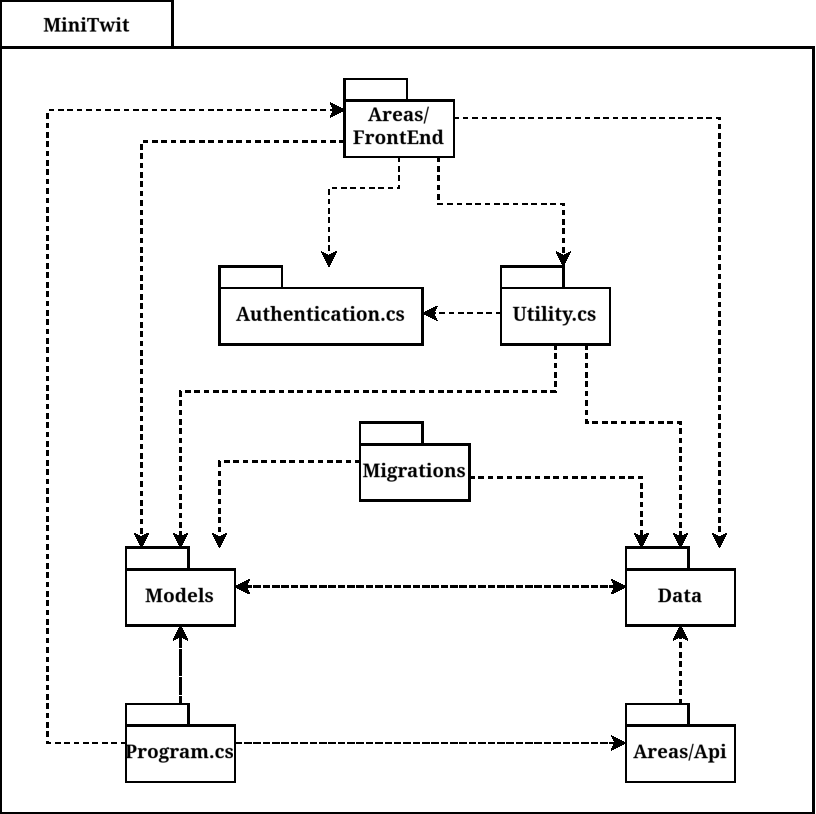
\includegraphics[width=0.50\textwidth]{module1.pdf}
	\end{center}
	\caption{Module view of the top-level modules of the MiniTwit application component.}\label{fig:module1}
\end{figure}




% !TeX encoding = UTF-8
% !TeX spellcheck = en_GB
\section{Systems dependencies}

The list below, is the technolgies we are using in our application, group into categories of technogy.

\subsection*{Project Start - choose framework}

\begin{itemize}
	\item Microsoft AspNetCore v2 as the foundational framework.
	\item Dotnet API framework: For handling RESTFul APIs
	\item Swagger: For dotnet API visualization
	\item Microsoft EntityFrameworkCore version 8.x: Secure and reliable data transactions
	\item Postgress v.8: Stable data storage
	\item Docker : For containerized applications
	\item gravatar: For generating user profile images.
	\item Github: For storing and deploying source code
	\item DigitalOcean: Production server for our application
\end{itemize}

\subsection*{Monitoring}

\begin{itemize}
	\item Prometheus: For providing metrics to Grafana.
	\item Grafana: For Data Visualization of data from prometheus and direct data from Postgress database.
\end{itemize}

\subsection*{Logging}

\begin{itemize}
	\item Serilog AspNetCore v.8: For logging.
	\item Fluentd: For collecting logs from different sources.
\end{itemize}


\subsection*{Software quality - Testing}

\begin{itemize}
	\item Sonarqube: Static analyzer for code quality and security issues
	\item CodeClimate: Another static analyzer also for code quality and securit issues
	\item Playwright: UI testing
	\item Cypress: End-2-end testing
	\item Xunit: For Basic Unit testing
\end{itemize}


\section{Systems Interactions}

This section the interations flow of request for the system, by user create a new request into the system. The request flow is create by providing sequence diagrams, of demostration for 4 important task for the system, namely, register a user, user login, user create a new tweet, and user follow another user. 



\begin{figure}[H]
	\centering
	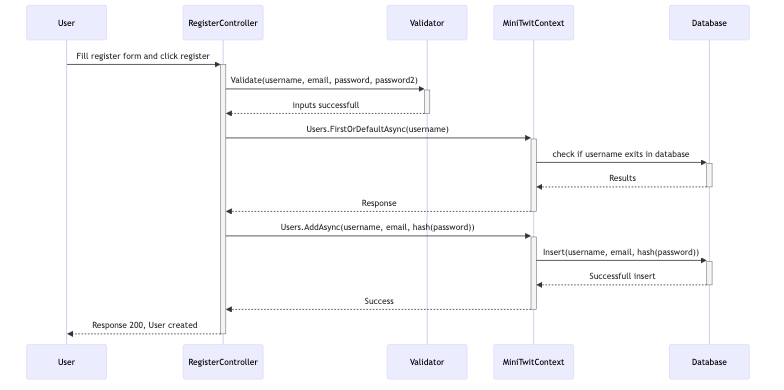
\includegraphics[width=0.75\textwidth]{register_sequence.png}
	\caption{Sequence diagram demostrate the flow of registerings of a user}
	\label{fig:register_sequence}
\end{figure}


\begin{figure}[H]
	\centering
	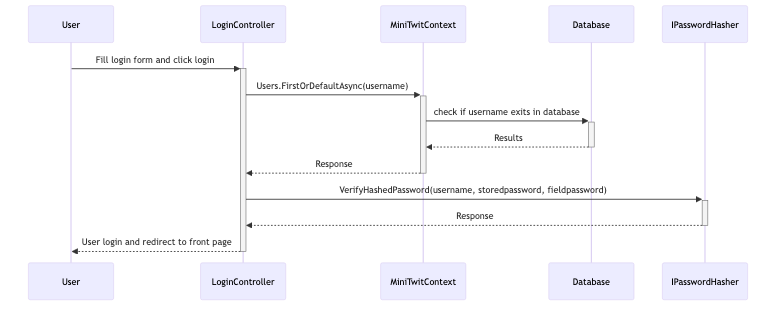
\includegraphics[width=0.75\textwidth]{login_sequence.png}
	\caption{Sequence diagram demostrate the login procedure for a user}
	\label{fig:login_sequence}
\end{figure}

\begin{figure}[H]
	\centering
	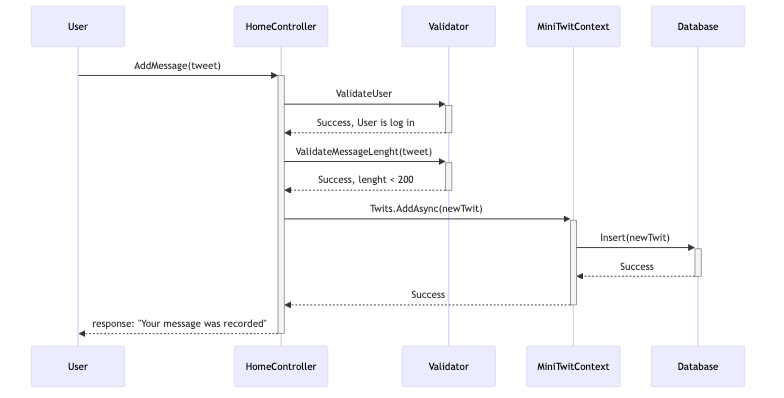
\includegraphics[width=0.75\textwidth]{twit_sequence.png}
	\caption{Sequence diagram demostrate the procedure for create a new twit}
	\label{fig:twit_sequence}
\end{figure}

\begin{figure}[H]
	\centering
	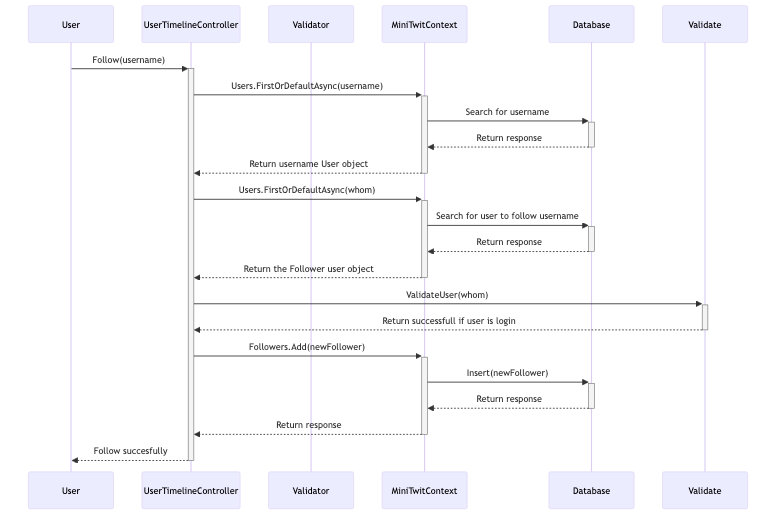
\includegraphics[width=0.75\textwidth]{follow_sequence.png}
	\caption{Sequence diagram of the procedure for a user follow another user}
	\label{fig:follow_sequence}
\end{figure}


\section{Current state of our application}

We have use Sonarqube and codeclimate to analyze our code base. This section will describe the current state of our application, acording to the two analyze tools. 

\subsection*{Codeclimate}

\begin{figure}[h]
	\centering
	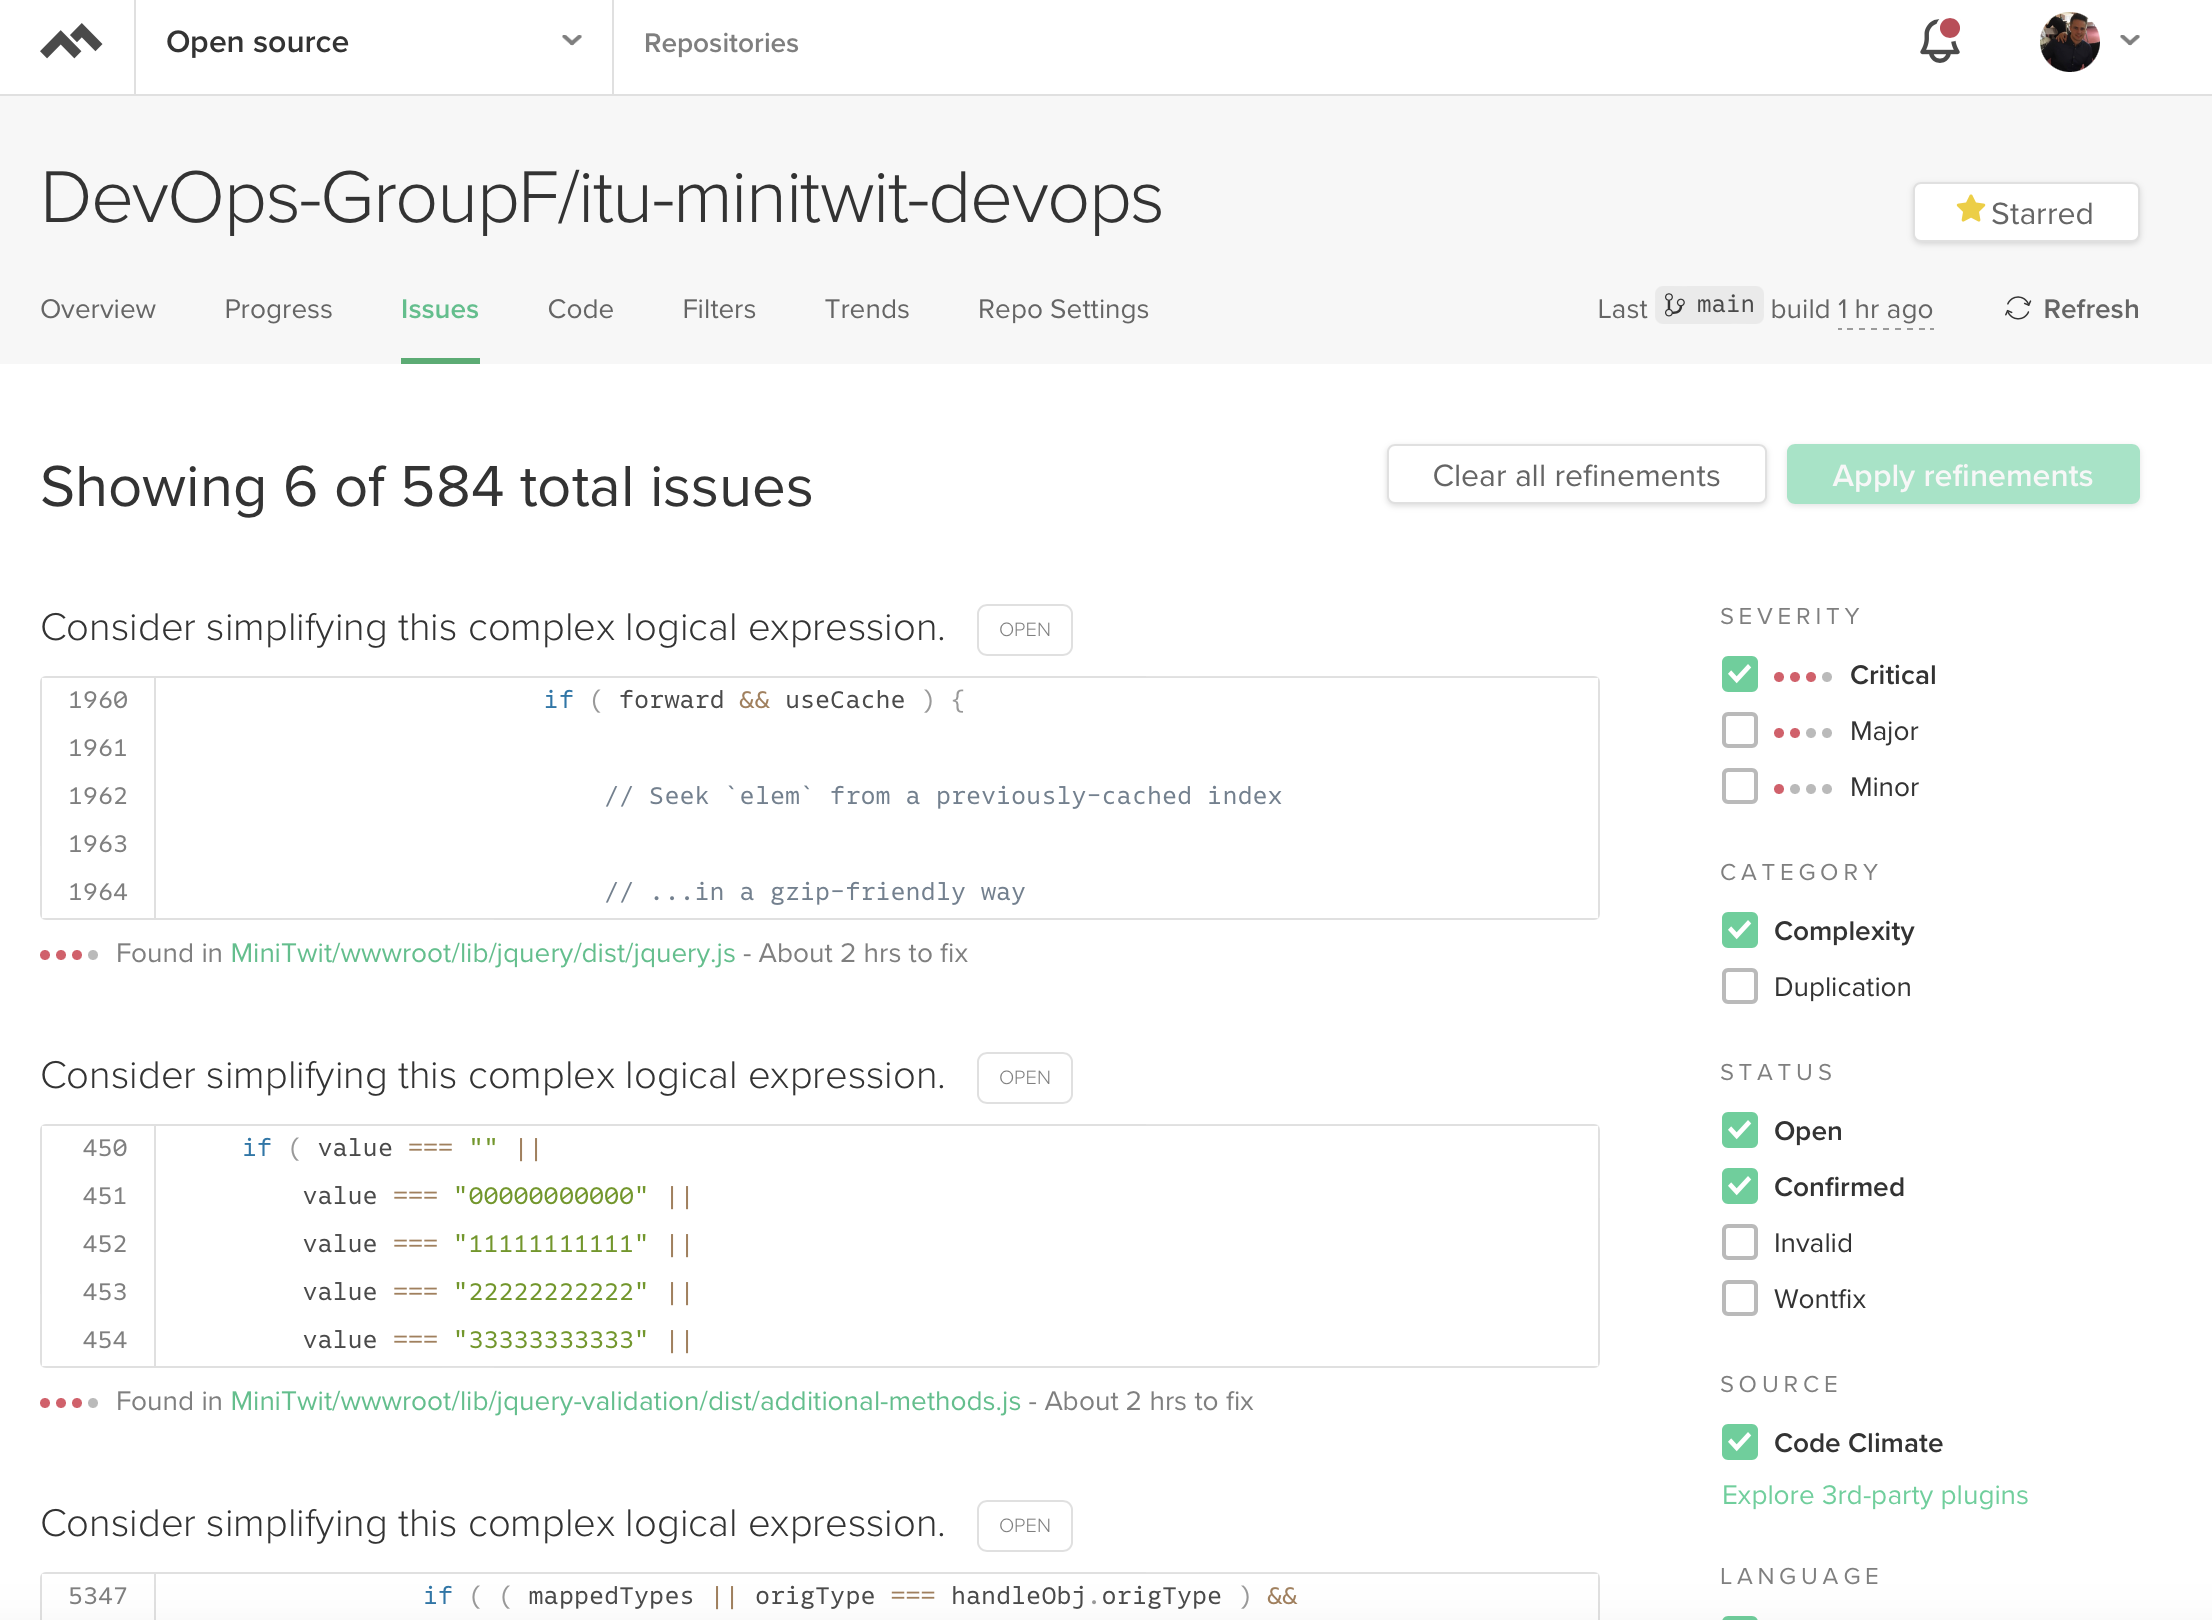
\includegraphics[width=0.75\textwidth]{codeclitemate.png}
	\caption{Code climate report}
	\label{fig:Code climate}
\end{figure}

Codeclimate general reports 323 code smells, and 261 duplication. Mostly of these is from the javascript lib we are using, for some reason even try to filter code, so only \texttt{C\#} code is shown, it still include it. Also it was also possible to filter critical issues, here were 6 found, but related to our used third party javascript library jquery. So nothing we can do here. 

\subsection*{Sonarqube}
Sunarqube report several issues. Mostly it report security issues, because we are logging to much in our application, which could cause security issues. 
\begin{figure}[h]
	\centering
	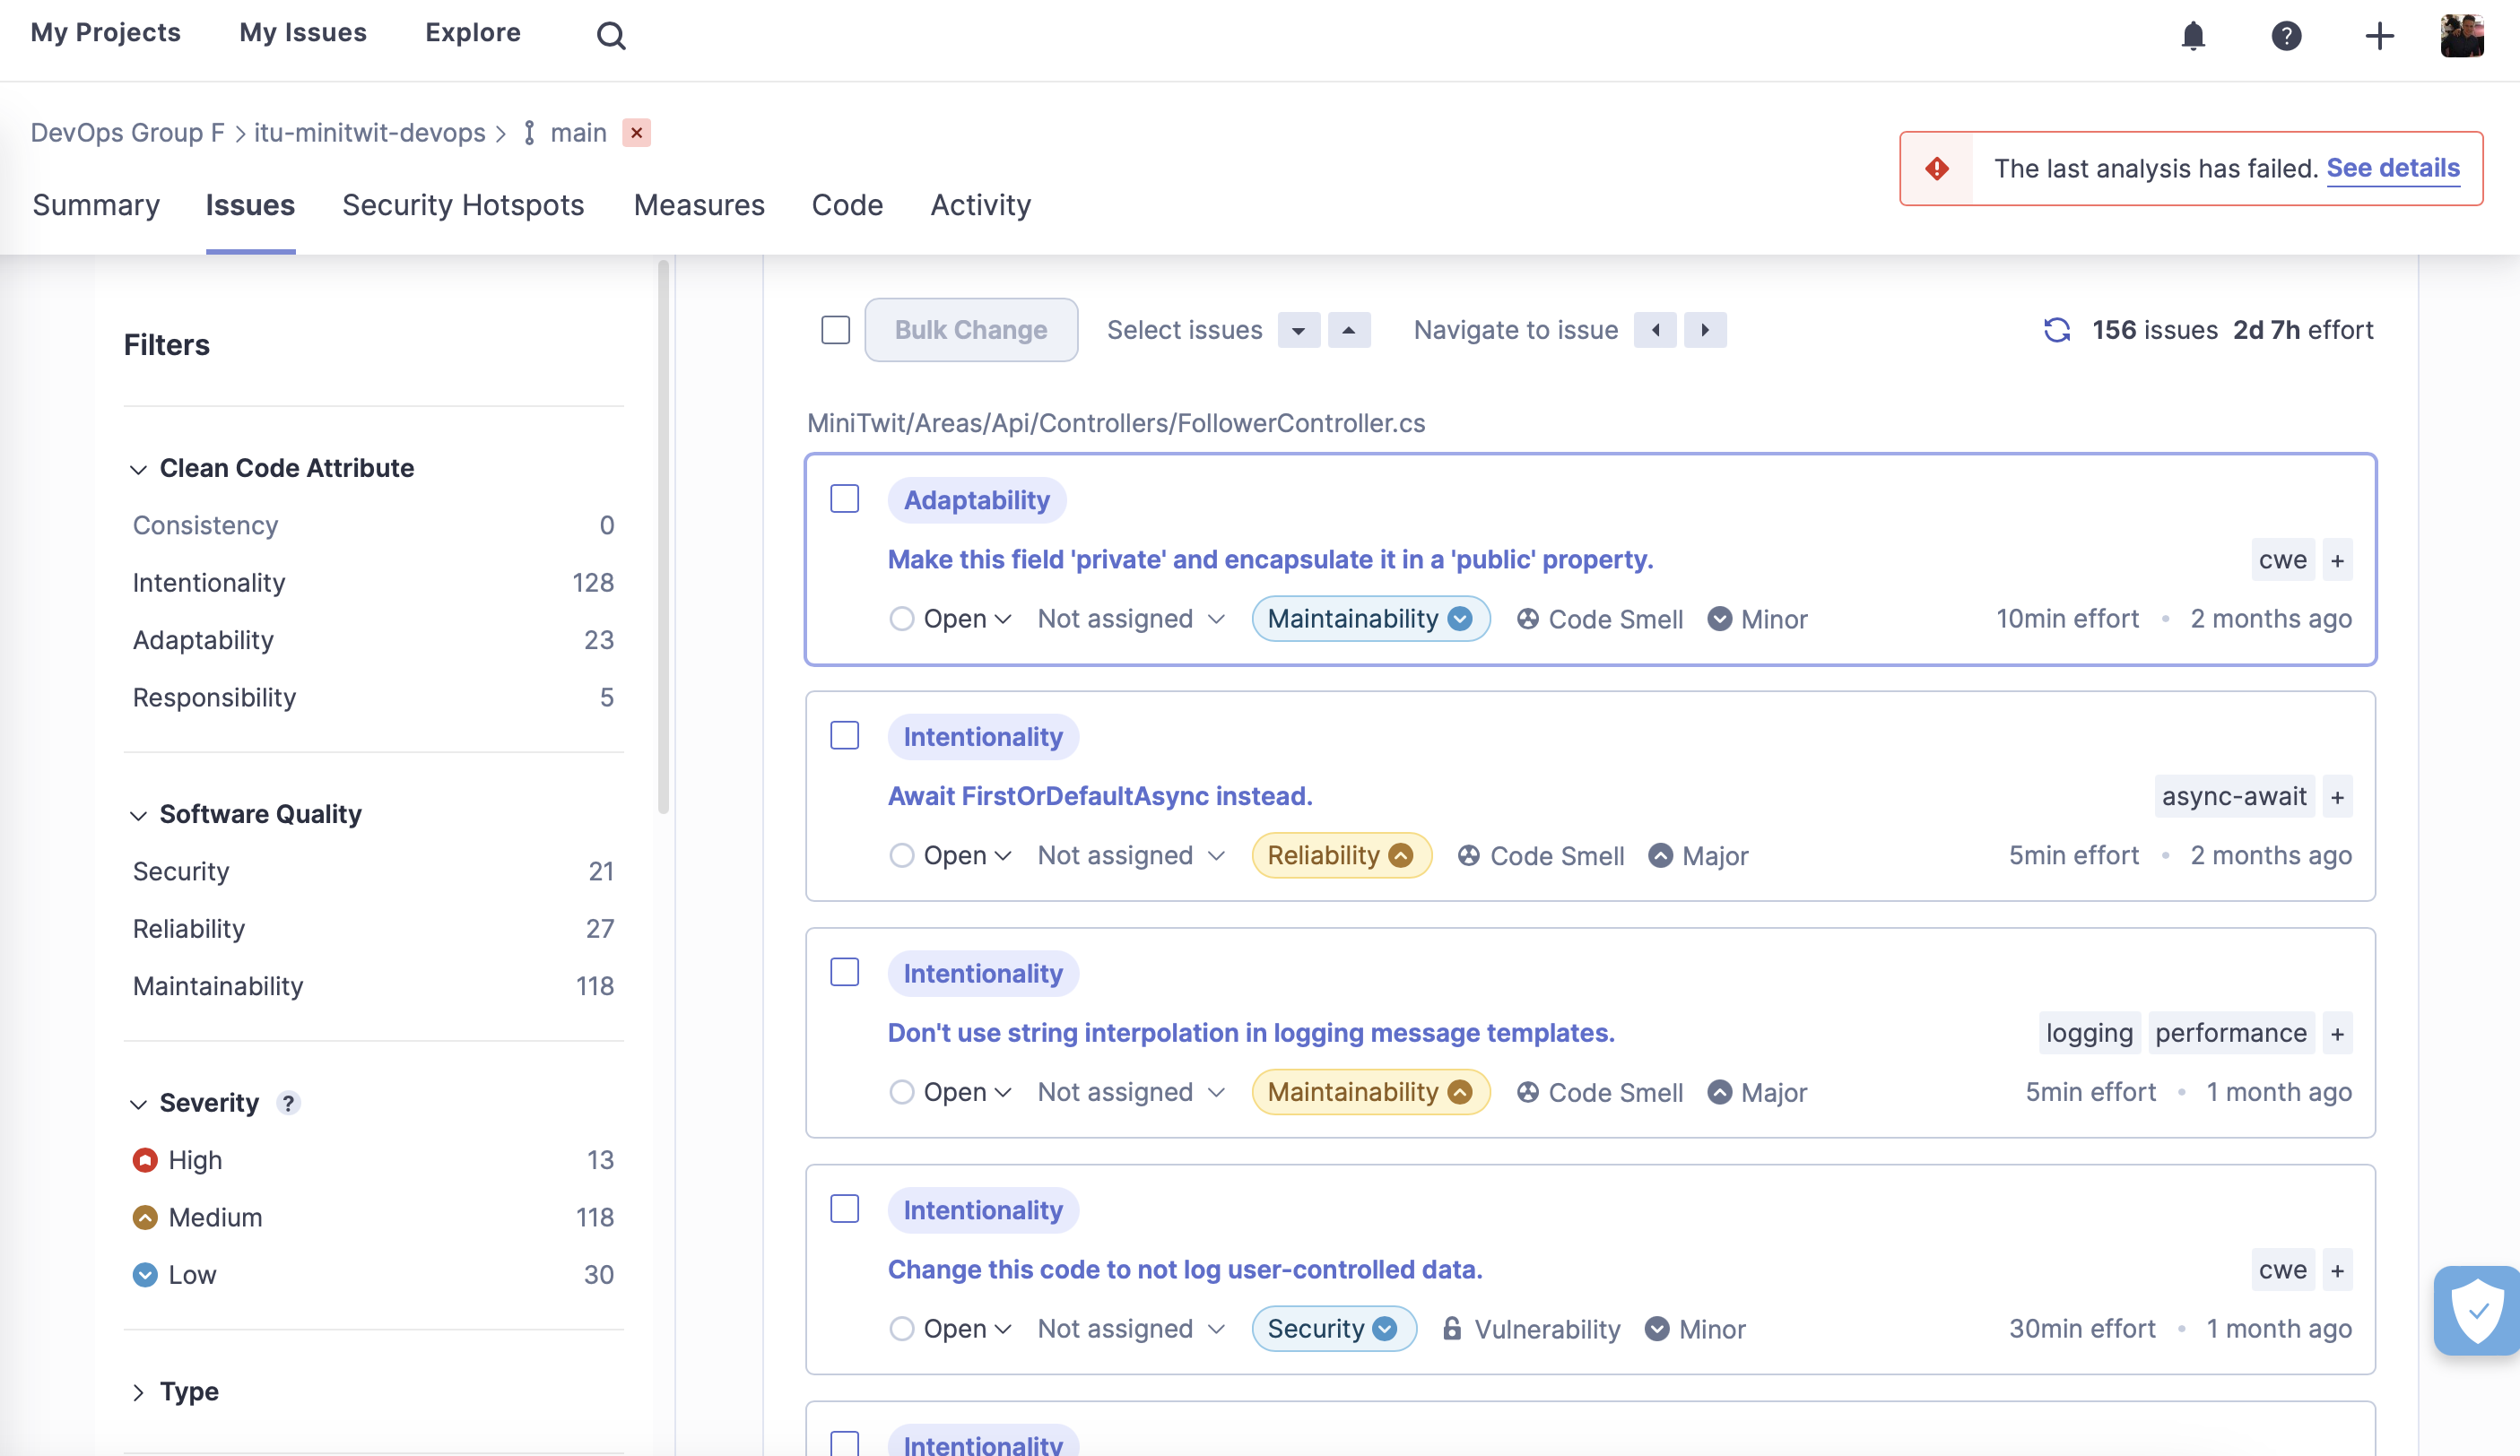
\includegraphics[width=0.75\textwidth]{sonarqube.png}
	\caption{Sonarqube report}
	\label{fig:Sonarqube}
\end{figure}
